\documentclass[11pt,a4paper,roman]{moderncv}        % possible options include font size ('10pt', '11pt' and '12pt'), paper size ('a4paper', 'letterpaper', 'a5paper', 'legalpaper', 'executivepaper' and 'landscape') and font family ('sans' and 'roman')

% moderncv themes
\moderncvstyle{banking}                            % style options are 'casual' (default), 'classic', 'oldstyle' and 'banking'
\moderncvcolor{blue}                                % color options 'blue' (default), 'orange', 'green', 'red', 'purple', 'grey' and 'black'
\renewcommand{\familydefault}{\rmdefault}         % to set the default font; use '\sfdefault' for the default sans serif font, '\rmdefault' for the default roman one, or any tex font name
\nopagenumbers{}                                  % uncomment to suppress automatic page numbering for CVs longer than one page

% character encoding
\usepackage[utf8]{inputenc}                       % if you are not using xelatex ou lualatex, replace by the encoding you are using
%\usepackage{CJKutf8}                              % if you need to use CJK to typeset your resume in Chinese, Japanese or Korean

% adjust the page margins
\usepackage[scale=0.75]{geometry}
%\setlength{\hintscolumnwidth}{3cm}                % if you want to change the width of the column with the dates
%\setlength{\makecvtitlenamewidth}{10cm}           % for the 'classic' style, if you want to force the width allocated to your name and avoid line breaks. be careful though, the length is normally calculated to avoid any overlap with your personal info; use this at your own typographical risks...

% personal data
\name{Hoa}{Nguyen-Thanh}
\title{Teaching Assistant and Master Student}                               % optional, remove / comment the line if not wanted
\address{University of Information Technology}{Vietnam National University (VNU-HCM)}{Ho Chi Minh City - Vietnam}% optional, remove / comment the line if not wanted; the "postcode city" and and "country" arguments can be omitted or provided empty
\phone[mobile]{+84~833~221293}                   % optional, remove / comment the line if not wanted
%\phone[fixed]{+2~(345)~678~901}                    % optional, remove / comment the line if not wanted
%\phone[fax]{+3~(456)~789~012}                      % optional, remove / comment the line if not wanted
\email{hoant@uit.edu.vn}                               % optional, remove / comment the line if not wanted
\homepage{linkedin.com/in/nguyenthanhhoa}                         % optional, remove / comment the line if not wanted
%\extrainfo{Teaching Assistant and Master student}                 % optional, remove / comment the line if not wanted
%\photo[90pt][0pt]{picture}                       % optional, remove / comment the line if not wanted; '64pt' is the height the picture must be resized to, 0.4pt is the thickness of the frame around it (put it to 0pt for no frame) and 'picture' is the name of the picture file
%\quote{\textbf{Teaching Assistant and Master student}}                                 % optional, remove / comment the line if not wanted


%%%%%title and name on different lines
\usepackage{xpatch}
\makeatletter
\xpatchcmd\makehead
   {\titlestyle{~|~\@title}}%
   {\par\vskip1ex\titlestyle{\@title}}%
   {}{}
\makeatother

%%%%%% Change title font size (\namefont \titlefont, \addressfont, \quotefont, \sectionfont, \subsectionfont, \hintfont and \pagenumberfont.)
\renewcommand*{\titlefont}{\fontsize{15}{15}\mdseries\upshape}

% to show numerical labels in the bibliography (default is to show no labels); only useful if you make citations in your resume
%\makeatletter
%\renewcommand*{\bibliographyitemlabel}{\@biblabel{\arabic{enumiv}}}
%\makeatother
%\renewcommand*{\bibliographyitemlabel}{[\arabic{enumiv}]}% CONSIDER REPLACING THE ABOVE BY THIS

% bibliography with mutiple entries
%\usepackage{multibib}
%\newcites{book,misc}{{Books},{Others}}
%----------------------------------------------------------------------------------
%            content
%----------------------------------------------------------------------------------
\begin{document}

%\begin{picture}(0,0)
%\put(380,-60){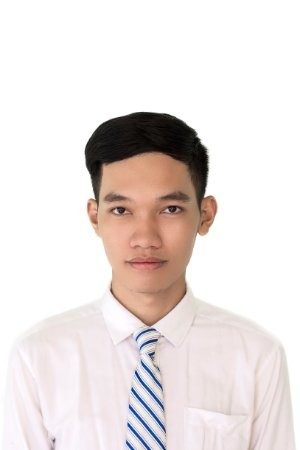
\includegraphics[scale=0.35]{picture}}
%\end{picture}
%-----       resume       ---------------------------------------------------------
\makecvtitle

\section{Education}
\cventry{2011-2016}{Undergraduate Degree}{University of Information Technology - VNU-HCM}{Ho Chi Minh City}{\textit{GPA: \textbf{9.02}/10}}
{Major: Computer Networks and Communications
\\ Thesis: "Build management and control system for surveillance cameras with Raspberry Pi"
\\ Advisor: Dr. Tuan \textsc{Nguyen-Anh} - Grade: \textbf{9.4}/10\\}  % arguments 3 to 6 can be left empty

\cventry{2016 - current}{Master Degree}{University of Information Technology - VNU-HCM}{Ho Chi Minh City}{\textit{GPA: \textbf{8.97}/10}}{Major: Computer Science}

\section{Research Interest}
\cvitem{Principal research interests}{\emph{computer network}}
Master student in Computer Science at University of Information Technology (VNU-HCM), seeking to leverage two study abroad experiences and a semester-long research internship to undertake postgraduate research regarding future networks. 


\section{Experience}
\subsection{Vocational}
\cventry{year--year}{Job title}{Employer}{City}{}{General description no longer than 1--2 lines.\newline{}%
Detailed achievements:%
\begin{itemize}%
\item Achievement 1;
\item Achievement 2, with sub-achievements:
  \begin{itemize}%
  \item Sub-achievement (a);
  \item Sub-achievement (b), with sub-sub-achievements (don't do this!);
    \begin{itemize}
    \item Sub-sub-achievement i;
    \item Sub-sub-achievement ii;
    \item Sub-sub-achievement iii;
    \end{itemize}
  \item Sub-achievement (c);
  \end{itemize}
\item Achievement 3.
\end{itemize}}
\cventry{year--year}{Job title}{Employer}{City}{}{Description line 1\newline{}Description line 2}
\subsection{Miscellaneous}
\cventry{year--year}{Job title}{Employer}{City}{}{Description}

\section{Languages}
\cvitemwithcomment{Language 1}{Skill level}{Comment}
\cvitemwithcomment{Language 2}{Skill level}{Comment}
\cvitemwithcomment{Language 3}{Skill level}{Comment}

\section{Computer skills}
\cvdoubleitem{category 1}{XXX, YYY, ZZZ}{category 4}{XXX, YYY, ZZZ}
\cvdoubleitem{category 2}{XXX, YYY, ZZZ}{category 5}{XXX, YYY, ZZZ}
\cvdoubleitem{category 3}{XXX, YYY, ZZZ}{category 6}{XXX, YYY, ZZZ}

\section{Extra 2}
\cvlistdoubleitem{Item 1}{Item 4}
\cvlistdoubleitem{Item 2}{Item 5\cite{book1}}
\cvlistdoubleitem{Item 3}{Item 6. Like item 3 in the single column list before, this item is particularly long to wrap over several lines.}

\section{References}
\begin{cvcolumns}
  \cvcolumn{Category 1}{\begin{itemize}\item Person 1\item Person 2\item Person 3\end{itemize}}
  \cvcolumn{Category 2}{Amongst others:\begin{itemize}\item Person 1, and\item Person 2\end{itemize}(more upon request)}
  \cvcolumn[0.5]{All the rest \& some more}{\textit{That} person, and \textbf{those} also (all available upon request).}
\end{cvcolumns}

% Publications from a BibTeX file without multibib
%  for numerical labels: \renewcommand{\bibliographyitemlabel}{\@biblabel{\arabic{enumiv}}}% CONSIDER MERGING WITH PREAMBLE PART
%  to redefine the heading string ("Publications"): \renewcommand{\refname}{Articles}
\nocite{*}
\bibliographystyle{plain}
\bibliography{publications}                        % 'publications' is the name of a BibTeX file

% Publications from a BibTeX file using the multibib package
%\section{Publications}
%\nocitebook{book1,book2}
%\bibliographystylebook{plain}
%\bibliographybook{publications}                   % 'publications' is the name of a BibTeX file
%\nocitemisc{misc1,misc2,misc3}
%\bibliographystylemisc{plain}
%\bibliographymisc{publications}                   % 'publications' is the name of a BibTeX file
\end{document}


%% end of file `template.tex'.